% Created by tikzDevice version 0.12.3.1 on 2023-05-05 12:20:04
% !TEX encoding = UTF-8 Unicode
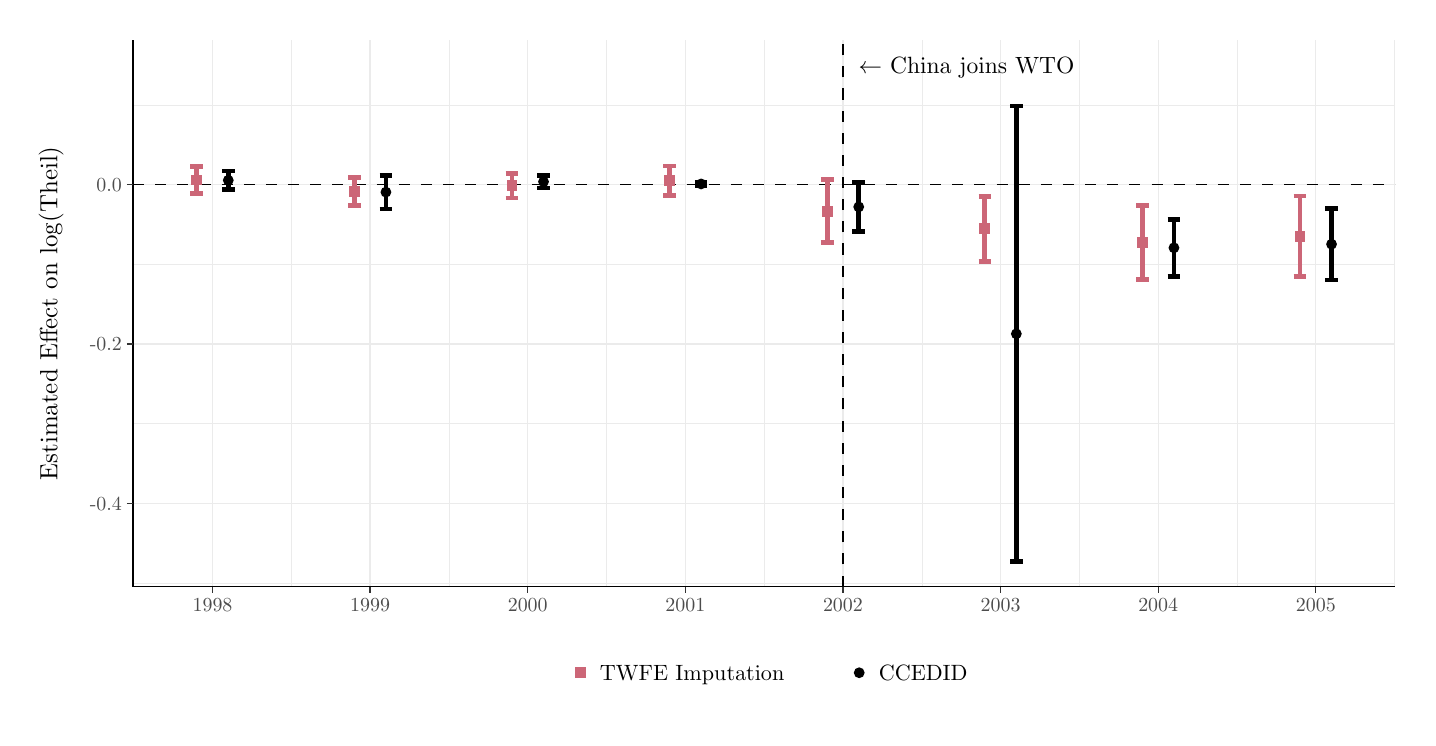
\begin{tikzpicture}[x=1pt,y=1pt]
\definecolor{fillColor}{RGB}{255,255,255}
\path[use as bounding box,fill=fillColor,fill opacity=0.00] (0,0) rectangle (498.66,249.33);
\begin{scope}
\path[clip] (  0.00,  0.00) rectangle (498.66,249.33);
\definecolor{drawColor}{RGB}{255,255,255}
\definecolor{fillColor}{RGB}{255,255,255}

\path[draw=drawColor,line width= 0.5pt,line join=round,line cap=round,fill=fillColor] ( -0.00,  0.00) rectangle (498.66,249.33);
\end{scope}
\begin{scope}
\path[clip] ( 38.10, 47.36) rectangle (494.16,244.83);
\definecolor{fillColor}{RGB}{255,255,255}

\path[fill=fillColor] ( 38.10, 47.36) rectangle (494.16,244.83);
\definecolor{drawColor}{gray}{0.92}

\path[draw=drawColor,line width= 0.2pt,line join=round] ( 38.10, 48.65) --
	(494.16, 48.65);

\path[draw=drawColor,line width= 0.2pt,line join=round] ( 38.10,106.25) --
	(494.16,106.25);

\path[draw=drawColor,line width= 0.2pt,line join=round] ( 38.10,163.85) --
	(494.16,163.85);

\path[draw=drawColor,line width= 0.2pt,line join=round] ( 38.10,221.45) --
	(494.16,221.45);

\path[draw=drawColor,line width= 0.2pt,line join=round] ( 38.32, 47.36) --
	( 38.32,244.83);

\path[draw=drawColor,line width= 0.2pt,line join=round] ( 95.27, 47.36) --
	( 95.27,244.83);

\path[draw=drawColor,line width= 0.2pt,line join=round] (152.23, 47.36) --
	(152.23,244.83);

\path[draw=drawColor,line width= 0.2pt,line join=round] (209.18, 47.36) --
	(209.18,244.83);

\path[draw=drawColor,line width= 0.2pt,line join=round] (266.13, 47.36) --
	(266.13,244.83);

\path[draw=drawColor,line width= 0.2pt,line join=round] (323.08, 47.36) --
	(323.08,244.83);

\path[draw=drawColor,line width= 0.2pt,line join=round] (380.03, 47.36) --
	(380.03,244.83);

\path[draw=drawColor,line width= 0.2pt,line join=round] (436.98, 47.36) --
	(436.98,244.83);

\path[draw=drawColor,line width= 0.2pt,line join=round] (493.94, 47.36) --
	(493.94,244.83);

\path[draw=drawColor,line width= 0.5pt,line join=round] ( 38.10, 77.45) --
	(494.16, 77.45);

\path[draw=drawColor,line width= 0.5pt,line join=round] ( 38.10,135.05) --
	(494.16,135.05);

\path[draw=drawColor,line width= 0.5pt,line join=round] ( 38.10,192.65) --
	(494.16,192.65);

\path[draw=drawColor,line width= 0.5pt,line join=round] ( 66.80, 47.36) --
	( 66.80,244.83);

\path[draw=drawColor,line width= 0.5pt,line join=round] (123.75, 47.36) --
	(123.75,244.83);

\path[draw=drawColor,line width= 0.5pt,line join=round] (180.70, 47.36) --
	(180.70,244.83);

\path[draw=drawColor,line width= 0.5pt,line join=round] (237.65, 47.36) --
	(237.65,244.83);

\path[draw=drawColor,line width= 0.5pt,line join=round] (294.60, 47.36) --
	(294.60,244.83);

\path[draw=drawColor,line width= 0.5pt,line join=round] (351.56, 47.36) --
	(351.56,244.83);

\path[draw=drawColor,line width= 0.5pt,line join=round] (408.51, 47.36) --
	(408.51,244.83);

\path[draw=drawColor,line width= 0.5pt,line join=round] (465.46, 47.36) --
	(465.46,244.83);
\definecolor{drawColor}{RGB}{0,0,0}

\path[draw=drawColor,line width= 0.6pt,dash pattern=on 4pt off 4pt ,line join=round] ( 38.10,192.65) -- (494.16,192.65);

\path[draw=drawColor,line width= 0.6pt,dash pattern=on 4pt off 4pt ,line join=round] (294.60, 47.36) -- (294.60,244.83);

\node[text=drawColor,anchor=base west,inner sep=0pt, outer sep=0pt, scale=  0.85] at (300.30,232.92) {$\leftarrow$ China joins WTO};
\definecolor{drawColor}{RGB}{204,102,119}

\path[draw=drawColor,line width= 1.7pt,line join=round] ( 58.83,199.24) --
	( 63.38,199.24);

\path[draw=drawColor,line width= 1.7pt,line join=round] ( 61.10,199.24) --
	( 61.10,189.39);

\path[draw=drawColor,line width= 1.7pt,line join=round] ( 58.83,189.39) --
	( 63.38,189.39);

\path[draw=drawColor,line width= 1.7pt,line join=round] (115.78,195.14) --
	(120.33,195.14);

\path[draw=drawColor,line width= 1.7pt,line join=round] (118.06,195.14) --
	(118.06,185.17);

\path[draw=drawColor,line width= 1.7pt,line join=round] (115.78,185.17) --
	(120.33,185.17);

\path[draw=drawColor,line width= 1.7pt,line join=round] (172.73,196.57) --
	(177.28,196.57);

\path[draw=drawColor,line width= 1.7pt,line join=round] (175.01,196.57) --
	(175.01,187.81);

\path[draw=drawColor,line width= 1.7pt,line join=round] (172.73,187.81) --
	(177.28,187.81);

\path[draw=drawColor,line width= 1.7pt,line join=round] (229.68,199.33) --
	(234.24,199.33);

\path[draw=drawColor,line width= 1.7pt,line join=round] (231.96,199.33) --
	(231.96,188.60);

\path[draw=drawColor,line width= 1.7pt,line join=round] (229.68,188.60) --
	(234.24,188.60);

\path[draw=drawColor,line width= 1.7pt,line join=round] (286.63,194.34) --
	(291.19,194.34);

\path[draw=drawColor,line width= 1.7pt,line join=round] (288.91,194.34) --
	(288.91,171.69);

\path[draw=drawColor,line width= 1.7pt,line join=round] (286.63,171.69) --
	(291.19,171.69);

\path[draw=drawColor,line width= 1.7pt,line join=round] (343.58,188.35) --
	(348.14,188.35);

\path[draw=drawColor,line width= 1.7pt,line join=round] (345.86,188.35) --
	(345.86,164.88);

\path[draw=drawColor,line width= 1.7pt,line join=round] (343.58,164.88) --
	(348.14,164.88);

\path[draw=drawColor,line width= 1.7pt,line join=round] (400.53,185.03) --
	(405.09,185.03);

\path[draw=drawColor,line width= 1.7pt,line join=round] (402.81,185.03) --
	(402.81,158.25);

\path[draw=drawColor,line width= 1.7pt,line join=round] (400.53,158.25) --
	(405.09,158.25);

\path[draw=drawColor,line width= 1.7pt,line join=round] (457.49,188.51) --
	(462.04,188.51);

\path[draw=drawColor,line width= 1.7pt,line join=round] (459.76,188.51) --
	(459.76,159.48);

\path[draw=drawColor,line width= 1.7pt,line join=round] (457.49,159.48) --
	(462.04,159.48);
\definecolor{drawColor}{RGB}{0,0,0}

\path[draw=drawColor,line width= 1.7pt,line join=round] ( 70.22,197.53) --
	( 74.77,197.53);

\path[draw=drawColor,line width= 1.7pt,line join=round] ( 72.49,197.53) --
	( 72.49,190.83);

\path[draw=drawColor,line width= 1.7pt,line join=round] ( 70.22,190.83) --
	( 74.77,190.83);

\path[draw=drawColor,line width= 1.7pt,line join=round] (127.17,195.96) --
	(131.72,195.96);

\path[draw=drawColor,line width= 1.7pt,line join=round] (129.45,195.96) --
	(129.45,183.84);

\path[draw=drawColor,line width= 1.7pt,line join=round] (127.17,183.84) --
	(131.72,183.84);

\path[draw=drawColor,line width= 1.7pt,line join=round] (184.12,195.93) --
	(188.68,195.93);

\path[draw=drawColor,line width= 1.7pt,line join=round] (186.40,195.93) --
	(186.40,191.43);

\path[draw=drawColor,line width= 1.7pt,line join=round] (184.12,191.43) --
	(188.68,191.43);

\path[draw=drawColor,line width= 1.7pt,line join=round] (241.07,193.32) --
	(245.63,193.32);

\path[draw=drawColor,line width= 1.7pt,line join=round] (243.35,193.32) --
	(243.35,192.40);

\path[draw=drawColor,line width= 1.7pt,line join=round] (241.07,192.40) --
	(245.63,192.40);

\path[draw=drawColor,line width= 1.7pt,line join=round] (298.02,193.36) --
	(302.58,193.36);

\path[draw=drawColor,line width= 1.7pt,line join=round] (300.30,193.36) --
	(300.30,175.78);

\path[draw=drawColor,line width= 1.7pt,line join=round] (298.02,175.78) --
	(302.58,175.78);

\path[draw=drawColor,line width= 1.7pt,line join=round] (354.97,221.05) --
	(359.53,221.05);

\path[draw=drawColor,line width= 1.7pt,line join=round] (357.25,221.05) --
	(357.25, 56.34);

\path[draw=drawColor,line width= 1.7pt,line join=round] (354.97, 56.34) --
	(359.53, 56.34);

\path[draw=drawColor,line width= 1.7pt,line join=round] (411.92,180.07) --
	(416.48,180.07);

\path[draw=drawColor,line width= 1.7pt,line join=round] (414.20,180.07) --
	(414.20,159.52);

\path[draw=drawColor,line width= 1.7pt,line join=round] (411.92,159.52) --
	(416.48,159.52);

\path[draw=drawColor,line width= 1.7pt,line join=round] (468.88,184.02) --
	(473.43,184.02);

\path[draw=drawColor,line width= 1.7pt,line join=round] (471.15,184.02) --
	(471.15,158.16);

\path[draw=drawColor,line width= 1.7pt,line join=round] (468.88,158.16) --
	(473.43,158.16);
\definecolor{fillColor}{RGB}{204,102,119}

\path[fill=fillColor] ( 59.14,192.35) --
	( 63.07,192.35) --
	( 63.07,196.27) --
	( 59.14,196.27) --
	cycle;

\path[fill=fillColor] (116.09,188.19) --
	(120.02,188.19) --
	(120.02,192.11) --
	(116.09,192.11) --
	cycle;

\path[fill=fillColor] (173.04,190.23) --
	(176.97,190.23) --
	(176.97,194.15) --
	(173.04,194.15) --
	cycle;

\path[fill=fillColor] (230.00,192.00) --
	(233.92,192.00) --
	(233.92,195.93) --
	(230.00,195.93) --
	cycle;

\path[fill=fillColor] (286.95,181.05) --
	(290.87,181.05) --
	(290.87,184.98) --
	(286.95,184.98) --
	cycle;

\path[fill=fillColor] (343.90,174.65) --
	(347.82,174.65) --
	(347.82,178.58) --
	(343.90,178.58) --
	cycle;

\path[fill=fillColor] (400.85,169.68) --
	(404.77,169.68) --
	(404.77,173.60) --
	(400.85,173.60) --
	cycle;

\path[fill=fillColor] (457.80,172.04) --
	(461.73,172.04) --
	(461.73,175.96) --
	(457.80,175.96) --
	cycle;
\definecolor{fillColor}{RGB}{0,0,0}

\path[fill=fillColor] ( 72.49,194.18) circle (  1.96);

\path[fill=fillColor] (129.45,189.90) circle (  1.96);

\path[fill=fillColor] (186.40,193.68) circle (  1.96);

\path[fill=fillColor] (243.35,192.86) circle (  1.96);

\path[fill=fillColor] (300.30,184.57) circle (  1.96);

\path[fill=fillColor] (357.25,138.70) circle (  1.96);

\path[fill=fillColor] (414.20,169.79) circle (  1.96);

\path[fill=fillColor] (471.15,171.09) circle (  1.96);
\end{scope}
\begin{scope}
\path[clip] (  0.00,  0.00) rectangle (498.66,249.33);
\definecolor{drawColor}{RGB}{0,0,0}

\path[draw=drawColor,line width= 0.5pt,line join=round] ( 38.10, 47.36) --
	( 38.10,244.83);
\end{scope}
\begin{scope}
\path[clip] (  0.00,  0.00) rectangle (498.66,249.33);
\definecolor{drawColor}{gray}{0.30}

\node[text=drawColor,anchor=base east,inner sep=0pt, outer sep=0pt, scale=  0.72] at ( 34.05, 74.97) {-0.4};

\node[text=drawColor,anchor=base east,inner sep=0pt, outer sep=0pt, scale=  0.72] at ( 34.05,132.57) {-0.2};

\node[text=drawColor,anchor=base east,inner sep=0pt, outer sep=0pt, scale=  0.72] at ( 34.05,190.17) {0.0};
\end{scope}
\begin{scope}
\path[clip] (  0.00,  0.00) rectangle (498.66,249.33);
\definecolor{drawColor}{gray}{0.20}

\path[draw=drawColor,line width= 0.5pt,line join=round] ( 35.85, 77.45) --
	( 38.10, 77.45);

\path[draw=drawColor,line width= 0.5pt,line join=round] ( 35.85,135.05) --
	( 38.10,135.05);

\path[draw=drawColor,line width= 0.5pt,line join=round] ( 35.85,192.65) --
	( 38.10,192.65);
\end{scope}
\begin{scope}
\path[clip] (  0.00,  0.00) rectangle (498.66,249.33);
\definecolor{drawColor}{RGB}{0,0,0}

\path[draw=drawColor,line width= 0.5pt,line join=round] ( 38.10, 47.36) --
	(494.16, 47.36);
\end{scope}
\begin{scope}
\path[clip] (  0.00,  0.00) rectangle (498.66,249.33);
\definecolor{drawColor}{gray}{0.20}

\path[draw=drawColor,line width= 0.5pt,line join=round] ( 66.80, 45.11) --
	( 66.80, 47.36);

\path[draw=drawColor,line width= 0.5pt,line join=round] (123.75, 45.11) --
	(123.75, 47.36);

\path[draw=drawColor,line width= 0.5pt,line join=round] (180.70, 45.11) --
	(180.70, 47.36);

\path[draw=drawColor,line width= 0.5pt,line join=round] (237.65, 45.11) --
	(237.65, 47.36);

\path[draw=drawColor,line width= 0.5pt,line join=round] (294.60, 45.11) --
	(294.60, 47.36);

\path[draw=drawColor,line width= 0.5pt,line join=round] (351.56, 45.11) --
	(351.56, 47.36);

\path[draw=drawColor,line width= 0.5pt,line join=round] (408.51, 45.11) --
	(408.51, 47.36);

\path[draw=drawColor,line width= 0.5pt,line join=round] (465.46, 45.11) --
	(465.46, 47.36);
\end{scope}
\begin{scope}
\path[clip] (  0.00,  0.00) rectangle (498.66,249.33);
\definecolor{drawColor}{gray}{0.30}

\node[text=drawColor,anchor=base,inner sep=0pt, outer sep=0pt, scale=  0.72] at ( 66.80, 38.35) {1998};

\node[text=drawColor,anchor=base,inner sep=0pt, outer sep=0pt, scale=  0.72] at (123.75, 38.35) {1999};

\node[text=drawColor,anchor=base,inner sep=0pt, outer sep=0pt, scale=  0.72] at (180.70, 38.35) {2000};

\node[text=drawColor,anchor=base,inner sep=0pt, outer sep=0pt, scale=  0.72] at (237.65, 38.35) {2001};

\node[text=drawColor,anchor=base,inner sep=0pt, outer sep=0pt, scale=  0.72] at (294.60, 38.35) {2002};

\node[text=drawColor,anchor=base,inner sep=0pt, outer sep=0pt, scale=  0.72] at (351.56, 38.35) {2003};

\node[text=drawColor,anchor=base,inner sep=0pt, outer sep=0pt, scale=  0.72] at (408.51, 38.35) {2004};

\node[text=drawColor,anchor=base,inner sep=0pt, outer sep=0pt, scale=  0.72] at (465.46, 38.35) {2005};
\end{scope}
\begin{scope}
\path[clip] (  0.00,  0.00) rectangle (498.66,249.33);
\definecolor{drawColor}{RGB}{0,0,0}

\node[text=drawColor,rotate= 90.00,anchor=base,inner sep=0pt, outer sep=0pt, scale=  0.90] at ( 10.70,146.10) {Estimated Effect on $\log($Theil$)$};
\end{scope}
\begin{scope}
\path[clip] (  0.00,  0.00) rectangle (498.66,249.33);
\definecolor{fillColor}{RGB}{255,255,255}

\path[fill=fillColor] (178.11,  4.50) rectangle (354.15, 27.95);
\end{scope}
\begin{scope}
\path[clip] (  0.00,  0.00) rectangle (498.66,249.33);
\definecolor{fillColor}{RGB}{255,255,255}

\path[fill=fillColor] (185.45,  9.00) rectangle (213.91, 23.45);
\end{scope}
\begin{scope}
\path[clip] (  0.00,  0.00) rectangle (498.66,249.33);
\definecolor{fillColor}{RGB}{204,102,119}

\path[fill=fillColor] (197.72, 14.26) --
	(201.64, 14.26) --
	(201.64, 18.19) --
	(197.72, 18.19) --
	cycle;
\end{scope}
\begin{scope}
\path[clip] (  0.00,  0.00) rectangle (498.66,249.33);
\definecolor{fillColor}{RGB}{255,255,255}

\path[fill=fillColor] (286.25,  9.00) rectangle (314.70, 23.45);
\end{scope}
\begin{scope}
\path[clip] (  0.00,  0.00) rectangle (498.66,249.33);
\definecolor{fillColor}{RGB}{0,0,0}

\path[fill=fillColor] (300.47, 16.23) circle (  1.96);
\end{scope}
\begin{scope}
\path[clip] (  0.00,  0.00) rectangle (498.66,249.33);
\definecolor{drawColor}{RGB}{0,0,0}

\node[text=drawColor,anchor=base west,inner sep=0pt, outer sep=0pt, scale=  0.80] at (206.75, 13.47) {TWFE Imputation};
\end{scope}
\begin{scope}
\path[clip] (  0.00,  0.00) rectangle (498.66,249.33);
\definecolor{drawColor}{RGB}{0,0,0}

\node[text=drawColor,anchor=base west,inner sep=0pt, outer sep=0pt, scale=  0.80] at (307.55, 13.47) {CCEDID};
\end{scope}
\end{tikzpicture}
